\chapter{The Data and Associated Methods}

\section{Data Wrangling Methodology}
The data that forms the backbone of this project is courtesy of \cite{cricData}, which provides ball-by-ball match data for over 2000 One-Day International matches
and over 1500 Twenty20 matches. The ball-by-ball aspect of this data isn't immediately very useful, but the extra match information will be used extensively throught
this paper. Each match comes in the form of a .JSON file, so must be decoded first in order to make use of. All the code that will be discussed throught this section
can be found in appendix one. \newline


In order to get the data into a usable form, we wrote several Python programs to comb through and select datapoints that were of interest. Firstly, the data was split 
into games that were decided on DLS, and those that played out a full innings. This resulted in a CSV file containing information on 190 ODIs that were decided on DLS. 
The datapoints collected were the home and away team, the ground, the winner of the game, how much they won by, and what their target was. 
The rationale behind adding the ground is that the ground a game is played at has a considerable influence on how high a score will go. For example, 
consider the two grounds Edgbaston and Trent Bridge, in Birmingham and Nottingham respectively. The follwing table shows the averages of 6 international teams at the two 
English grounds in their entire ODI playing history.

%https://stats.espncricinfo.com/ci/engine/ground/56788.html?class=2;orderby=runs;template=results;type=aggregate
%https://stats.espncricinfo.com/ci/engine/ground/57219.html?class=2;orderby=runs;template=results;type=aggregate

\begin{center}
    \begin{tabular}{c|c|c}
    Team & Edgbaston Average & Trent Bridge Average \\
    \hline
    Australia & 196.3 & 272.9 \\  
    Bangladesh & 211.5 & 268.7 \\
    England & 227.8 & 246.1 \\
    India & 224.7 & 226.3 \\
    New Zealand & 202.2 & 241.9 \\
    Pakistan & 189.6 & 250.4 \\
    Overall & 208.7 & 251.1    
    \end{tabular}
\end{center}

So one can see that on average, a team playing at Trent Bridge is going to have a high scoring game than a team playing at Edgebaston. But this is something that DLS does
not take into account when revising the score. It is for this reason the ground has been included in the data. We also included the runs required to win, and how many overs
are available. Finally, we have how many runs or wickets the winning team won by. 

\section{Analysis of DLS Match Data}

We first look at the relationship betweem how many overs were available and how many runs required in those overs. The distubution of this can be seen in Figure 2.1.


\begin{figure}[t]
    \centering
    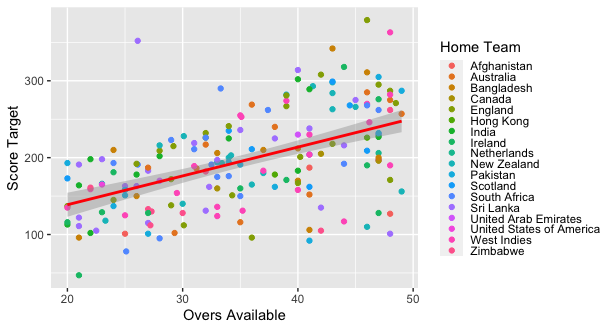
\includegraphics[scale=0.7]{figures/dlsOversScore.png}
    \caption{Distribution of Overs to Target, coloured by host nation }
    \label{figure 2.1}
\end{figure}

One thing that immediately sticks out is that there is a slight linear upward trend in the target score, but there is a considerable amount of variation in each over range. 
We have included a linear regression model, calculated in R using the \textit{lm()} function. The model given by this calculation is given as 

\begin{equation}
    R = 63.8 + 3.7O \pm 0.45.
\end{equation}

Where R is the number of runs required, and O is the overs available. So does that mean instead of going through the DLS process we could put overs into this model and read off the target score?
Well, no, because there is too much variation in target scores for this linear model to be reliable. To see this, we have a boxplot of the target runs produced by DLS. In the plot, each red cross 
represents a match.\footnote{Note that the vertical spread of points in this plot is purely a styalistic one}

\begin{figure}[h]
    \centering
    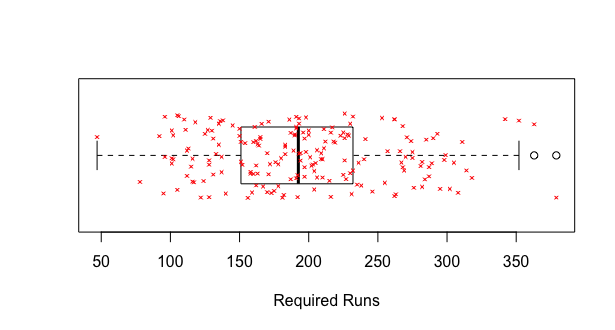
\includegraphics[scale=0.6]{figures/targetRunSpread.png}
    \caption{Distribution of target run scores calculated by DLS}
    \label{figure 2.2}
\end{figure}

If the two maximums were closer together, then this would arguably be a functional alternative to DLS, but the spread of scores is too large for the method to produce reliable results, and would often
result in a lot of targets that didn't fit with point (2) of the original 5 criteria. \newline

But how does the target score set by DLS compare with the actual data of successful run chases? We filter the data to include only successful target defences. The below data set shows data for the 112
games in which the team batting seccond were unable to reach their revised target, and how much the team batting first won by in the end.

\begin{figure}[h]
    \centering
    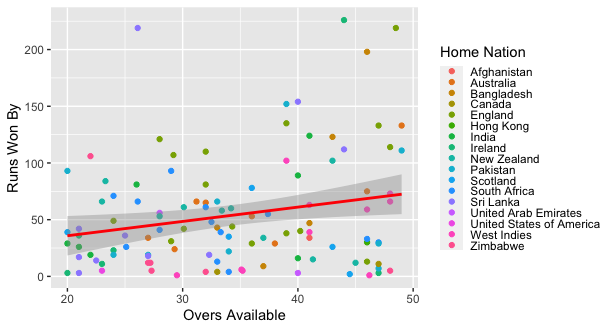
\includegraphics[scale=0.6]{figures/runsWonBy.png}
    \caption{Distribution of unssuccessful run chases}
    \label{figure 2.3}
\end{figure}

The linear regression model for figure 2.3 is give by:

\begin{equation}
    R = 10.6 + 1.26O \pm 0.52.
\end{equation}

One interesting thing of note here is that 6 games were won by over 150 runs. Two of these were in Sri Lanka, one in Pakistan and one in Bangladesh. Given the similar meteorological and ground conditions
in these nations, one could argue that the host nation should be taken into account when revising score targets?